\documentclass[a4paper,11pt]{article}
\usepackage[a4paper, margin=8em]{geometry}

% usa i pacchetti per la scrittura in italiano
\usepackage[french,italian]{babel}
\usepackage[T1]{fontenc}
\usepackage[utf8]{inputenc}
\frenchspacing 

% usa i pacchetti per la formattazione matematica
\usepackage{amsmath, amssymb, amsthm, amsfonts}

% usa altri pacchetti
\usepackage{gensymb}
\usepackage{hyperref}
\usepackage{standalone}

\usepackage{colortbl}

\usepackage{xstring}
\usepackage{karnaugh-map}

% imposta il titolo
\title{Appunti Sistemi Operativi}
\author{Luca Seggiani}
\date{2025}

% imposta lo stile
% usa helvetica
\usepackage[scaled]{helvet}
% usa palatino
\usepackage{palatino}
% usa un font monospazio guardabile
\usepackage{lmodern}

\renewcommand{\rmdefault}{ppl}
\renewcommand{\sfdefault}{phv}
\renewcommand{\ttdefault}{lmtt}

% circuiti
\usepackage{circuitikz}
\usetikzlibrary{babel}

% testo cerchiato
\newcommand*\circled[1]{\tikz[baseline=(char.base)]{
            \node[shape=circle,draw,inner sep=2pt] (char) {#1};}}

% disponi il titolo
\makeatletter
\renewcommand{\maketitle} {
	\begin{center} 
		\begin{minipage}[t]{.8\textwidth}
			\textsf{\huge\bfseries \@title} 
		\end{minipage}%
		\begin{minipage}[t]{.2\textwidth}
			\raggedleft \vspace{-1.65em}
			\textsf{\small \@author} \vfill
			\textsf{\small \@date}
		\end{minipage}
		\par
	\end{center}

	\thispagestyle{empty}
	\pagestyle{fancy}
}
\makeatother

% disponi teoremi
\usepackage{tcolorbox}
\newtcolorbox[auto counter, number within=section]{theorem}[2][]{%
	colback=blue!10, 
	colframe=blue!40!black, 
	sharp corners=northwest,
	fonttitle=\sffamily\bfseries, 
	title=Teorema~\thetcbcounter: #2, 
	#1
}

% disponi definizioni
\newtcolorbox[auto counter, number within=section]{definition}[2][]{%
	colback=red!10,
	colframe=red!40!black,
	sharp corners=northwest,
	fonttitle=\sffamily\bfseries,
	title=Definizione~\thetcbcounter: #2,
	#1
}

% disponi codice
\usepackage{listings}
\usepackage[table]{xcolor}

\definecolor{codegreen}{rgb}{0,0.6,0}
\definecolor{codegray}{rgb}{0.5,0.5,0.5}
\definecolor{codepurple}{rgb}{0.58,0,0.82}
\definecolor{backcolour}{rgb}{0.95,0.95,0.92}

\lstdefinestyle{codestyle}{
		backgroundcolor=\color{black!5}, 
		commentstyle=\color{codegreen},
		keywordstyle=\bfseries\color{magenta},
		numberstyle=\sffamily\tiny\color{black!60},
		stringstyle=\color{green!50!black},
		basicstyle=\ttfamily\footnotesize,
		breakatwhitespace=false,         
		breaklines=true,                 
		captionpos=b,                    
		keepspaces=true,                 
		numbers=left,                    
		numbersep=5pt,                  
		showspaces=false,                
		showstringspaces=false,
		showtabs=false,                  
		tabsize=2
}

\lstdefinestyle{shellstyle}{
		backgroundcolor=\color{black!5}, 
		basicstyle=\ttfamily\footnotesize\color{black}, 
		commentstyle=\color{black}, 
		keywordstyle=\color{black},
		numberstyle=\color{black!5},
		stringstyle=\color{black}, 
		showspaces=false,
		showstringspaces=false, 
		showtabs=false, 
		tabsize=2, 
		numbers=none, 
		breaklines=true
}


\lstdefinelanguage{assembler}{ 
  keywords={AAA, AAD, AAM, AAS, ADC, ADCB, ADCW, ADCL, ADD, ADDB, ADDW, ADDL, AND, ANDB, ANDW, ANDL,
        ARPL, BOUND, BSF, BSFL, BSFW, BSR, BSRL, BSRW, BSWAP, BT, BTC, BTCB, BTCW, BTCL, BTR, 
        BTRB, BTRW, BTRL, BTS, BTSB, BTSW, BTSL, CALL, CBW, CDQ, CLC, CLD, CLI, CLTS, CMC, CMP,
        CMPB, CMPW, CMPL, CMPS, CMPSB, CMPSD, CMPSW, CMPXCHG, CMPXCHGB, CMPXCHGW, CMPXCHGL,
        CMPXCHG8B, CPUID, CWDE, DAA, DAS, DEC, DECB, DECW, DECL, DIV, DIVB, DIVW, DIVL, ENTER,
        HLT, IDIV, IDIVB, IDIVW, IDIVL, IMUL, IMULB, IMULW, IMULL, IN, INB, INW, INL, INC, INCB,
        INCW, INCL, INS, INSB, INSD, INSW, INT, INT3, INTO, INVD, INVLPG, IRET, IRETD, JA, JAE,
        JB, JBE, JC, JCXZ, JE, JECXZ, JG, JGE, JL, JLE, JMP, JNA, JNAE, JNB, JNBE, JNC, JNE, JNG,
        JNGE, JNL, JNLE, JNO, JNP, JNS, JNZ, JO, JP, JPE, JPO, JS, JZ, LAHF, LAR, LCALL, LDS,
        LEA, LEAVE, LES, LFS, LGDT, LGS, LIDT, LMSW, LOCK, LODSB, LODSD, LODSW, LOOP, LOOPE,
        LOOPNE, LSL, LSS, LTR, MOV, MOVB, MOVW, MOVL, MOVSB, MOVSD, MOVSW, MOVSX, MOVSXB,
        MOVSXW, MOVSXL, MOVZX, MOVZXB, MOVZXW, MOVZXL, MUL, MULB, MULW, MULL, NEG, NEGB, NEGW,
        NEGL, NOP, NOT, NOTB, NOTW, NOTL, OR, ORB, ORW, ORL, OUT, OUTB, OUTW, OUTL, OUTSB, OUTSD,
        OUTSW, POP, POPL, POPW, POPB, POPA, POPAD, POPF, POPFD, PUSH, PUSHL, PUSHW, PUSHB, PUSHA, 
				PUSHAD, PUSHF, PUSHFD, RCL, RCLB, RCLW, MOVSL, MOVSB, MOVSW, STOSL, STOSB, STOSW, LODSB, LODSW,
				LODSL, INSB, INSW, INSL, OUTSB, OUTSL, OUTSW
        RCLL, RCR, RCRB, RCRW, RCRL, RDMSR, RDPMC, RDTSC, REP, REPE, REPNE, RET, ROL, ROLB, ROLW,
        ROLL, ROR, RORB, RORW, RORL, SAHF, SAL, SALB, SALW, SALL, SAR, SARB, SARW, SARL, SBB,
        SBBB, SBBW, SBBL, SCASB, SCASD, SCASW, SETA, SETAE, SETB, SETBE, SETC, SETE, SETG, SETGE,
        SETL, SETLE, SETNA, SETNAE, SETNB, SETNBE, SETNC, SETNE, SETNG, SETNGE, SETNL, SETNLE,
        SETNO, SETNP, SETNS, SETNZ, SETO, SETP, SETPE, SETPO, SETS, SETZ, SGDT, SHL, SHLB, SHLW,
        SHLL, SHLD, SHR, SHRB, SHRW, SHRL, SHRD, SIDT, SLDT, SMSW, STC, STD, STI, STOSB, STOSD,
        STOSW, STR, SUB, SUBB, SUBW, SUBL, TEST, TESTB, TESTW, TESTL, VERR, VERW, WAIT, WBINVD,
        XADD, XADDB, XADDW, XADDL, XCHG, XCHGB, XCHGW, XCHGL, XLAT, XLATB, XOR, XORB, XORW, XORL},
  keywordstyle=\color{blue}\bfseries,
  ndkeywordstyle=\color{darkgray}\bfseries,
  identifierstyle=\color{black},
  sensitive=false,
  comment=[l]{\#},
  morecomment=[s]{/*}{*/},
  commentstyle=\color{purple}\ttfamily,
  stringstyle=\color{red}\ttfamily,
  morestring=[b]',
  morestring=[b]"
}

\lstset{language=assembler, style=codestyle}

% disponi sezioni
\usepackage{titlesec}

\titleformat{\section}
	{\sffamily\Large\bfseries} 
	{\thesection}{1em}{} 
\titleformat{\subsection}
	{\sffamily\large\bfseries}   
	{\thesubsection}{1em}{} 
\titleformat{\subsubsection}
	{\sffamily\normalsize\bfseries} 
	{\thesubsubsection}{1em}{}

% tikz
\usepackage{tikz}

% float
\usepackage{float}

% grafici
\usepackage{pgfplots}
\pgfplotsset{width=10cm,compat=1.9}

% disponi alberi
\usepackage{forest}

\forestset{
	rectstyle/.style={
		for tree={rectangle,draw,font=\large\sffamily}
	},
	roundstyle/.style={
		for tree={circle,draw,font=\large}
	}
}

% disponi algoritmi
\usepackage{algorithm}
\usepackage{algorithmic}
\makeatletter
\renewcommand{\ALG@name}{Algoritmo}
\makeatother

% disponi numeri di pagina
\usepackage{fancyhdr}
\fancyhf{} 
\fancyfoot[L]{\sffamily{\thepage}}

\makeatletter
\fancyhead[L]{\raisebox{1ex}[0pt][0pt]{\sffamily{\@title \ \@date}}} 
\fancyhead[R]{\raisebox{1ex}[0pt][0pt]{\sffamily{\@author}}}
\makeatother

\begin{document}
% sezione (data)
\section{Lezione del 21-10-25}

% stili pagina
\thispagestyle{empty}
\pagestyle{fancy}

% testo
\subsection{Tassonomia di Flynn}
Prima di venire alla sincronizzazione dei processi, vediamo brevemente la \textbf{classificazione delle architetture} attraverso la \textit{tassonomia di Flynn}.

Questa è una classificazione che vede un sistema di elaborazione da 2 punti di vista ortogonali:
\begin{itemize}
	\item La capacità di avere più flussi di \textbf{esecuzione}: si possono distinguere \textbf{SI} (\textit{Single Instruction Stream}) e \textbf{MI} (\textit{Multiple Instruction Stream}). Questo concetto è vicino a quello di \textit{thread} visto nella scorsa sezione;
	\item La capacità di avere più flussi di \textbf{dati}: si possono distinguere \textbf{SD} (\textit{Single Data Stream}) e \textbf{MD} (\textit{Multiple Data Stream});
\end{itemize}

Abbiamo quindi la prima distinzione:
\begin{table}[H]
	\center \rowcolors{2}{white}{black!10}
	\begin{tabular} { p{3.5cm} || c | c  }
		& \bfseries SI (\textit{Single Instruction Stream}) & \bfseries MI (\textit{Multiple Instruction Stream}) \\
		\hline\hline
		\bfseries SD (\textit{Single Data Stream}) & Macchine SISD & Macchine MISD \\
		\bfseries MD (\textit{Multiple Data Stream}) & Macchine SIMD & Macchine MIMD \\
	\end{tabular}
\end{table}

Iniziamo a vedere dove si collocano le macchine che conosciamo.

\subsubsection{Macchine SISD}
Le macchine SISD rappresentano le tradizionali macchine \textit{sequenziali} e \textit{monoprocessore} definite dall'architettura di Von Neumann.
In questo caso si ha un solo flusso di istruzioni, ciascuna agente su al più un flusso dati, e ad ogni istante temporale si esegue una singola istruzione.

Vediamo una schematizzazione di questa architettura coerente con Flynn:
\begin{center}
	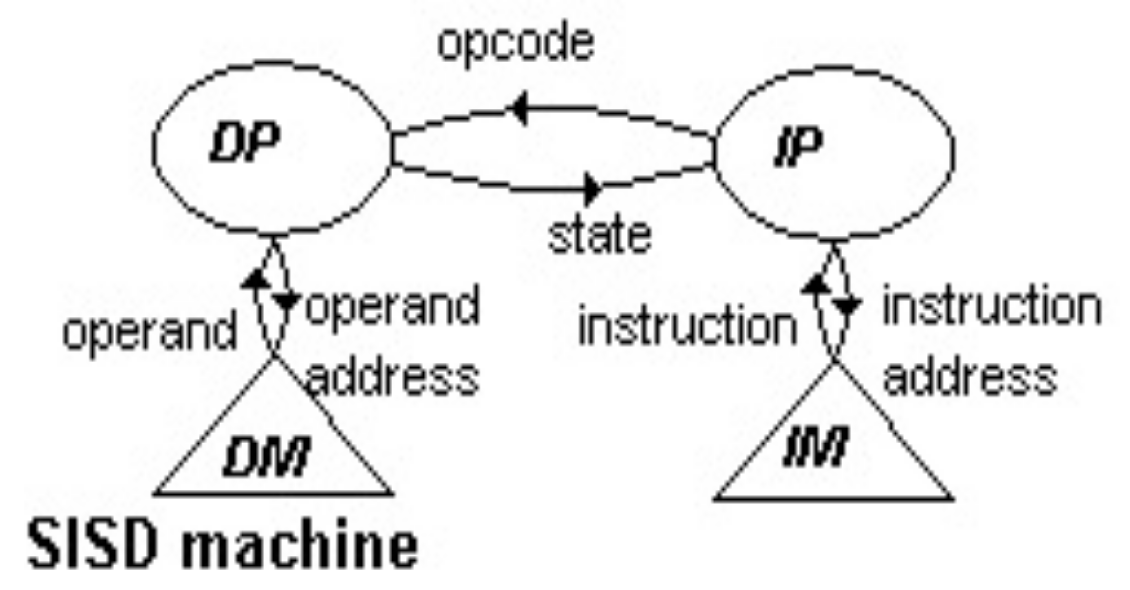
\includegraphics[scale=0.2]{../figures/sisd_flynn.png}
\end{center}

Da questa schematizzazione notiamo:
\begin{itemize}
	\item Un'unita di elaborazione \textbf{dati}, detta \textbf{DP} (\textit{Data Processor}), che interagisce ottenendo operandi e fornendo indirizzi di operandi (e sperabilmente dati) con uno stream \textbf{dati}, detto \textbf{DM} (\textit{Data Memory});
	\item Un'unità di elaborazione \textbf{istruzioni}, detta \textbf{IP} (\textit{Instruction Processor}), che interagisce ottenendo istruzioni e fornendo indirizzi di operazioni con uno stream \textbf{istruzioni}, detto \textbf{IM} (\textit{Instruction Memory}).
\end{itemize}

IP e DP interagiscono scambiandosi codifiche di istruzioni (IP $\rightarrow$ DP) e variazioni di stato (della memoria dati, DP $\rightarrow$ IP). 

Possiamo notare che la cosiddetta \textit{architettura Harvard} è un architettura che prevede, come dalla schematizzazione sopra, una forte separazione fra stream istruzioni e dati (di contro alla Von Neumann, che prevede un unica fonte di memoria per dati e istruzioni). 
Entrambe le architetture sono classificate come SISD, la Harvard è più usata in sistemi real-time mentre la Von Neumann è ancora oggi più usata nei sistemi general purpose.

\subsubsection{Macchine SIMD}
Le macchine SIMD sono formate da unità di elaborazione multiple, che eseguono le stesse istruzioni \textit{contemporaneamente}, ma su flussi di dati differenti.

\newpage

Una schematizzazione simile a quella sopra riportata è la seguente:
\begin{center}
	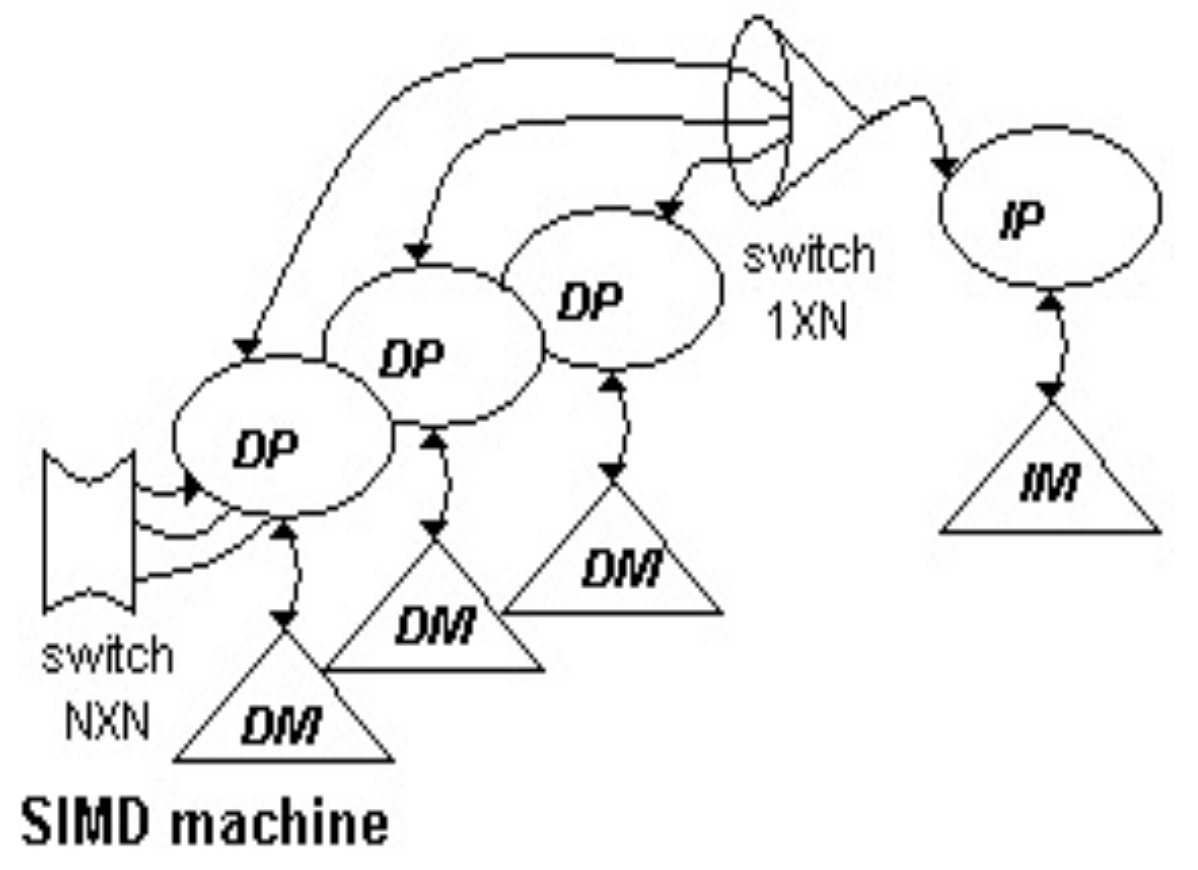
\includegraphics[scale=0.2]{../figures/simd_flynn.png}
\end{center}

Abbiamo che questa moltiplicazione dei flussi dati su cui si elabora si ha moltiplicando le unità di elaborazione dati (i \textbf{DP}), facendole obbedire ad una singola unità di elaborazione istruzion (l'\textbf{IP}).
Vediamo innanzitutto come si realizza la sincronizzazione fra questi DP: si prevede uno \textit{switch} $1\times N$ che porta le codifiche di istruzioni dall'IP a tutti i DP.

Per l'interazione fra le DP prevediamo poi uno switch $N \times N$ che le collega. Chiaramente questo switch sarà inefficiente, e vorremo usarlo il meno possibile.

Architetture di questo tipo possono essere \textit{regolari} o create \textit{ad hoc} sulla base della struttura del problema: nel caso di architetture regolari (cioè che rispettano la topologia fisica) non si hanno conflitti, e questo le rende efficienti e poco costose.

Le applicazioni di un'architettura di questo tipo sono nel caso di operazioni fortemente vettorizzate, come ad esempio nelle applicazioni grafiche e multimediali.
Inoltre, questo è il tipo di architettura che incontriamo spesso per macchine che devono portare avanti moli massiccie di computazione come i \textit{supercomputer}.

\par\smallskip

Riassumendo, possiamo dire che l'architettura SIMD prevede 2 tipi di parallelismo:
\begin{itemize}
	\item \textbf{Parallelismo temporale}: c'è un meccanismo di \textit{pipeline}, cioè fasi diverse di un’unica istruzione sono eseguite in parallelo in differenti moduli connessi in cascata.
	\item \textbf{Parallelismo spaziale}: i medesimi passi sono eseguiti contemporaneamente su un array di processori perfettamente uguali, sincronizzati da un solo controllore.
\end{itemize}

\par\smallskip

Lato programmatore possiamo prevedere due paradigmi per la compilazione di programmi pensati per l'esecuzione su macchine SIMD:
\begin{itemize}
	\item Il primo modo è non riscrivere il codice, sapendo che un programma pensato come scalare su macchina sequenziale (SISD), in esecuzione su macchina SIMD sarà vettoriale.

Avremo quindi che, ad esempio:
\begin{lstlisting}[language=C++, style=codestyle]	
// somma scalari
c = a + b
\end{lstlisting}
su macchina SIMD diventerà:
\begin{lstlisting}[language=C++, style=codestyle]	
// soma vettori (!)
C = A + B
\end{lstlisting}

	\item Nel caso si voglia essere più espliciti nel tipo di operazioni che facciamo, possiamo implementare un \textbf{compilatore vettoriale}: l'idea è che questo riconosca automaticamente quando le istruzioni SIMD potrebbero tornare utili per parallelizzare delle operazioni vettoriale, e inserisca quindi le operazioni necessarie.

		Ad esempio, potremmo volere:
\begin{lstlisting}[language=C++, style=codestyle]	
for(int i = 0; i < 100; i++) {
		c[i] = a[i] + b[i];
}
// qui riconosciamo che il ciclo e' vettorizzabile, e quindi lo vettorizziamo
\end{lstlisting}
\end{itemize}

\subsubsection{Macchine MISD}
In una macchina MISD vogliamo avere più flussi di istruzioni che lavorano contemporaneamente su un unico flusso dati.

Abbiamo che questa categoria è sostanzialmente vuota: il parallelismo fra più istruzioni in esecuzione sullo stesso flusso dati si ha effettivamente nei processori moderni solo attraverso il meccanismo della \textbf{pipeline}.

Se prevediamo che il processore debba svolgere per ogni istruzione più fasi, fra cui ad esempio:
\begin{enumerate}
	\item Prelievo istruzione;
	\item Decodifica;
	\item Prelievo operandi;
	\item Esecuzione;
	\item Scrittura.
\end{enumerate}
Avremo che questo potrà, disponendo di più unità di elaborazione atte a completare ognuna di queste fasi, parallelizzare come segue:
\begin{center}
	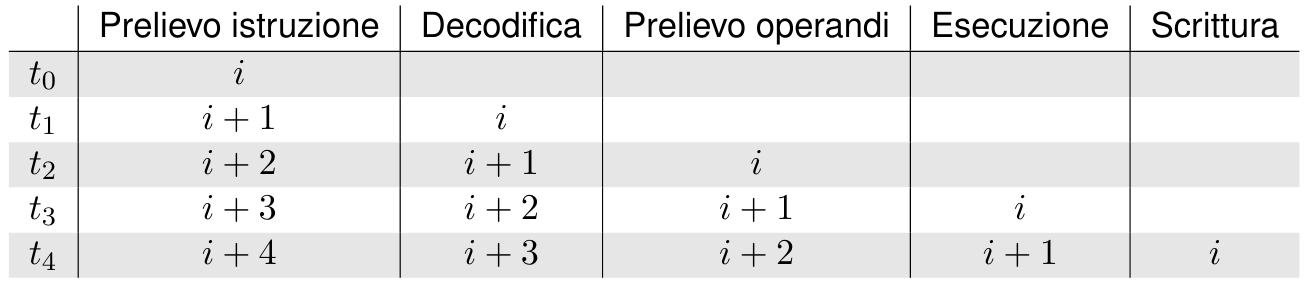
\includegraphics[scale=0.3]{../figures/pipeline.png}
\end{center}

In questo, a regime (nella tabella tempo $t_4$) si avranno più di un unità di elaborazione a lavoro contemporaneamente, e potremmo dire di aver realizzato in qualche modo il paradigma MISD.

Facciamo tra l'altro una nota sull'efficienza: se l'esecuzione di un'istruzione senza pipeline richiedeva un tempo $\Delta t$, e il troughput era $\frac{1}{T}$, prevedendo una pipeline ad $n$ stadi si riesce ad arrivare a $\frac{1}{T} \times n$ (assunto che ogni stadio richieda lo stesso tempo e si riesca a ridurre l'overhead dato da $n$ troppo grandi).

\subsubsection{Macchine MIMD}
Le macchine MIMD rappresentano per noi la categoria più interessante più flussi di istruzioni sono in esecuzione contemporaneamente su più processori, elaborando insiemi di dati distinti, privati o condivisi.

Ne prevediamo due tipologie principali:
\begin{itemize}
	\item \textbf{DM-MIMD} (\textit{Distributed Memory MIMD}), cioè a \textit{memoria distribuita}. Queste si schematizzano come segue:
\begin{center}
	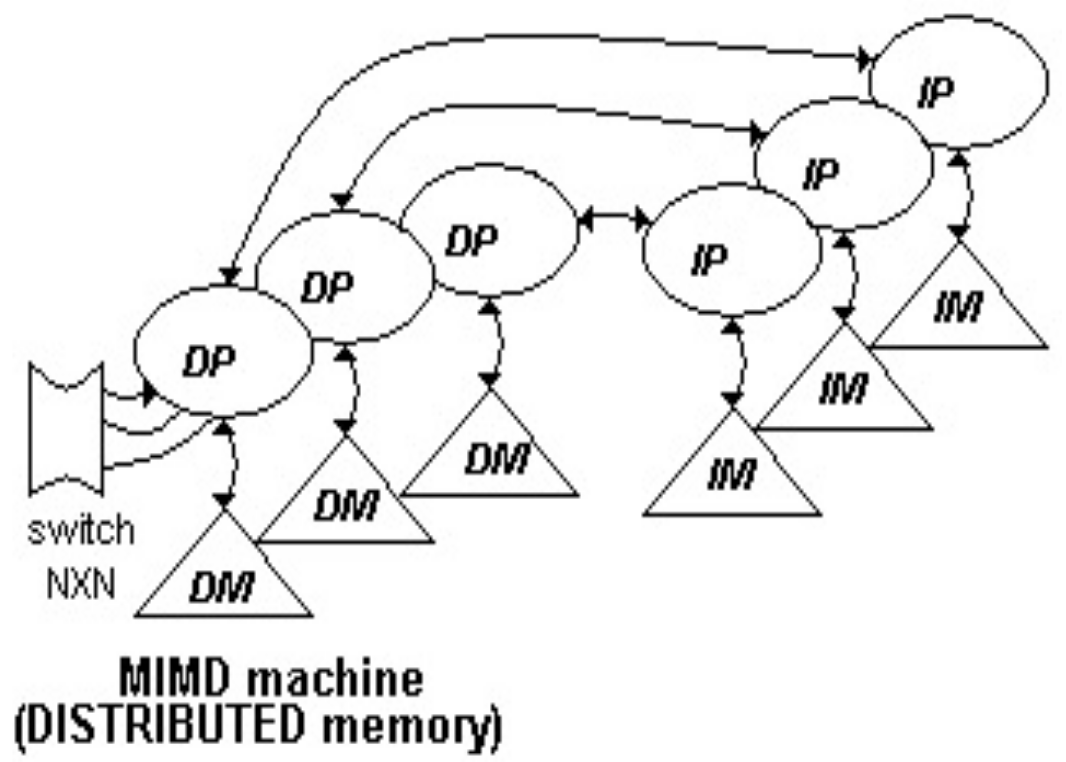
\includegraphics[scale=0.2]{../figures/dm-mimd.png}
\end{center}

In questo caso abbiamo più coppie IP-DP (con relative memorie IM e DM), che rappresentano sostanzialmente più macchine SISD. Uno switch $N \times N$ permette quindi la comunicazione fra le unità.

Abbiamo quindi che tra i nodi non esiste memoria condivisa e ogni nodo esegue indipendentemente un flusso di istruzioni su un differente insieme di dati, memorizzati su spazi differenti. La comunicazione è realizzata mediante una sottorete dedicata (appunto, lo switch).

Applicazioni di questa architettura sono ad esempio una qualsiasi \textit{rete di calcolatori} (come sia sviluppato lo switch non è specificato dal modello, e per noi potrebbe essere anche un router internet). 
Questo è il caso dei \textit{cluster} di workstation, realizzati solitamente attraverso \textit{Ethernet}. In questo richiediamo dalle macchine che compongono la rete 2 caratteristiche principali:
\begin{enumerate}
	\item \textbf{High-availability}: in caso di guasti, la computazione può migrare da un nodo all’altro;
	\item \textbf{Load-balancing}: i task da eseguire sono allocati nei nodi che hanno il minor carico.
\end{enumerate}

Architetture MIMD più stabili sono poi le rete di interconnessione regolari e dirette (ipercubi, mesh, torus), attraverso cui i nodi si scambiano informazioni secondo il paradigma del \textit{message passing} (\textit{"scambio di messaggi"}). Queste macchine sono molto scalabili e si prestano bene ad algoritmi ad elevata località: sono stati costruiti cluster composti anche da milioni di unità sequenziali.

\par\smallskip

Una variante del DM-MIMD è il \textbf{DM-MIMD MPP} (\textit{Massively Parallel Processing}). Questo è un paradigma utile in applicazioni scientifiche e particolari contesti di calcolo commerciale-finanziario. In un sistema MPP si ha:
\begin{itemize}
	\item Migliaia di nodi (CPU standard, ognuna con la propria memoria e la propria copia del SO)
	\item Una rete di interconnessione custom molto potente (larga banda e bassa latenza). Affinché l’elaborazione MPP dia effettivi vantaggi occorre disporre di software capace di partizionare il lavoro e i dati su cui opera tra i vari processori.
\end{itemize}

\item \textbf{SM-MIMD} (\textit{Single Memory MIMD}), cioè a \textit{memoria condivisa}. Queste si schematizzano come segue:
\begin{center}
	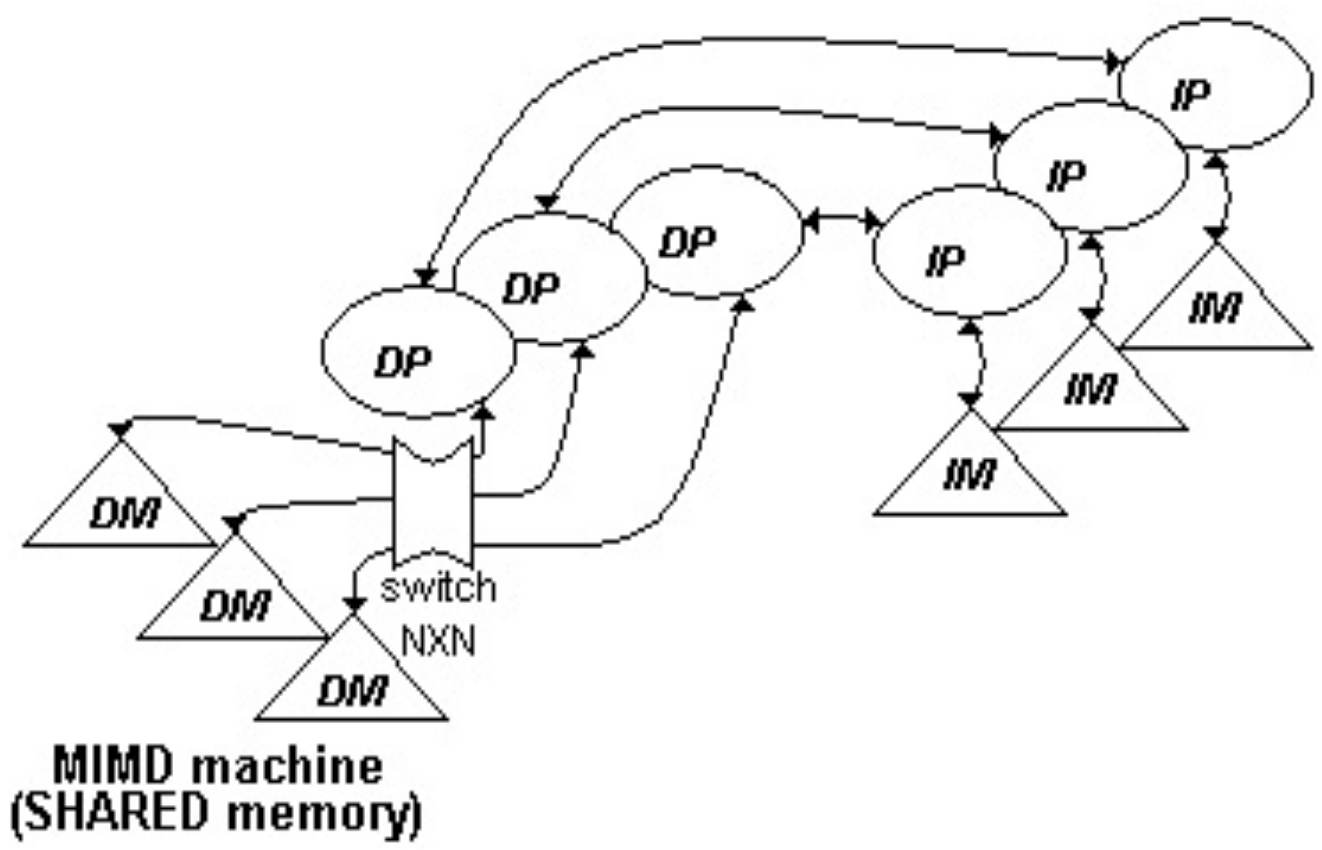
\includegraphics[scale=0.2]{../figures/sm-mimd.png}
\end{center}

Sono quindi macchine sempre \textit{multiprocessore}, ma dove le varie unità di elaborazione dati comunicano attraverso uno switch $N \times N$ con un \textit{pool} unico di memoria (formato anche da più flussi di memoria, ma visti allo stesso modo da ogni unità di elaborazione dati).

Questo approccio è meno scalabile, realizza la comunicazione fra processori condividendo aree di memoria, e richiede una rete di interconnessione (lo switch $N \times N$ estremamente efficiente).
Vogliamo che il numero $N$ di processori sia piccolo ($N < 100$), affiché si possa avere stretto accompiamento fra i nodi.
Si incorre chiaramente in problemi di competizione fra unità di elaborazione (mutua esclusione e sincronizzazione) che potrebbero impattare le prestazioni.
\end{itemize}

\subsubsection{Confronto fra SIMD e MIMD}
Possiamo fare quindi un confronto fra le architetture apperentemente simili, SIMD e MIMD:
\begin{itemize}
	\item Le SIMD richiedono meno hardware delle MIMD (c'è un unica unità di controllo, o \textit{elaborazione istruzioni});
	\item Le MIMD usano spesso processori general-purpose, quindi costano meno delle SIMD (che richiedono processori o ISA particolari, quindi meno hardware ma più specializzato);
	\item Le SIMD usano meno memoria delle MIMD (una sola copia del programma in memoria);
	\item Le MIMD godono di una grande flessibilità in termini di modelli computazionali supportati (si pensi \textit{client-server}, \textit{P2P}, ecc...). Di contro, è piuttosto semplice modificare un programma seqeunziale perché esegua su architettura SIMD in maniera vettorizzata.
\end{itemize}

\subsubsection{Sintesi della tassonomia di Flynn}
Possiamo quindi vedere un grafico riassuntivo delle tassonomie viste:
\begin{center}
	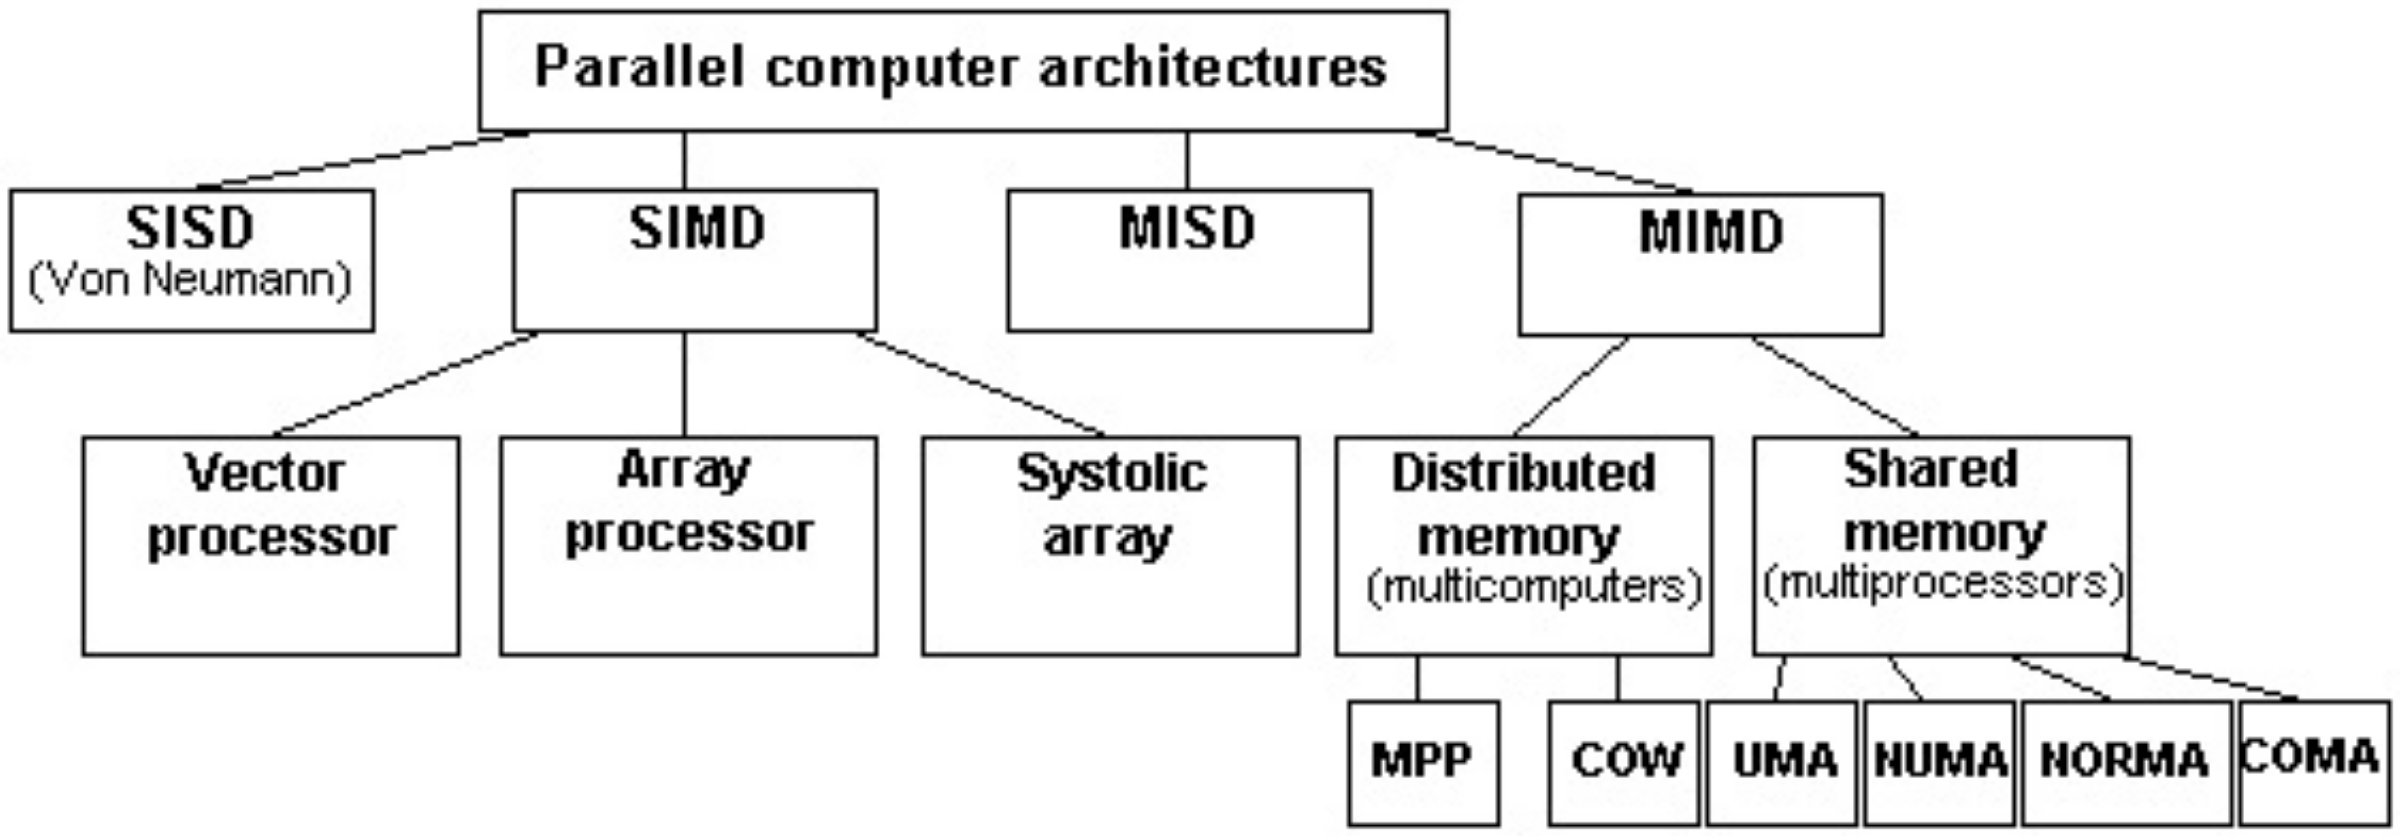
\includegraphics[scale=0.17]{../figures/flynn.png}
\end{center}

Dove si notano le 4 categorie principali (SISD, SIMD, MISD e MIMD) ed alcune sottocategorie (non abbiamo parlato di tutte le sottocategorie, per una trattazione più completa si rimanda alla letteratura).

\subsection{Tipologie di interconnessione}
Dopo aver discusso le architetture descritte dalla tassonomia di Flynn, vediamo i tipi principali di \textbf{interconnessione} che si possono avere fra unità di elaborazione (o in generale nodi).

\subsubsection{Bus}
\begin{center}
	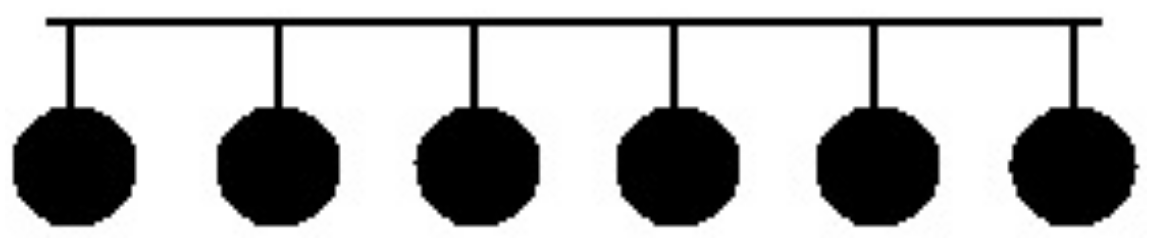
\includegraphics[scale=0.11]{../figures/bus.png}
\end{center}
Il \textbf{bus} è la più semplice rete di interconnessione che abbiamo visto.
Rappresenta una configurazione semplice ed affidabile (a meno che non si rompa il bus tutto funziona), dove ogni nodo a \textit{grado} 1 (tutti i nodi sono direttamente connessi al bus e a nient'altro), e il \textit{diametro} è 1 (la distanza massima è data dal solo bus).
Il numero totale di \textit{link} di cui abbiamo bisogno è sempre 1: il bus stesso è l'unico link di cui necessitiamo (i nodi devono solo collegarsi a tale link).

Il problema è chiaramente la \textit{competizione} sull'accesso al mezzo, che è massima: si hanno spesso problemi di mutua esclusione sulle stesse risorse, ad esempio quando più nodi vogliono accedere alla stessa risorsa contemporaneamente e devono farlo attraverso un unico bus.

\newpage

\subsubsection{Array lineare}
\begin{center}
	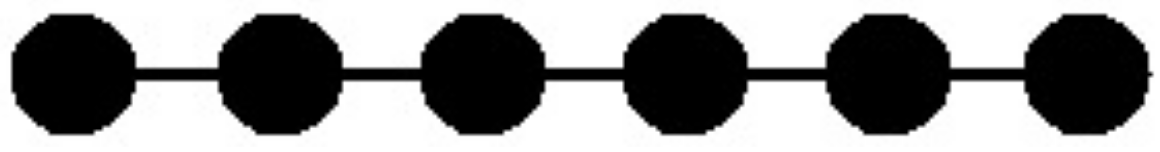
\includegraphics[scale=0.11]{../figures/linear.png}
\end{center}
L'\textbf{array lineare} espande in qualche modo l'idea del bus: in un certo senso vogliamo partizionare il bus in tanti link nodo a nodo. In questo caso il grado del primo e dell'ultimo nodo sarà 1, mentre quello dei restanti nodi sarà 2. Il diametro sara $n - 1$ per $n$ nodi, e il numero totale di link $n - 1$ (quelli necessari a legare ogni nodo con i nodi adiacenti).

Il vantaggio di questo approccio è la competizione, che viene ridotta al minimo (ogni coppia adiacente di nodi può comunicare indipendentemente dagli altri). Più nello specifico, nel caso ideale possiamo avere fino a $\frac{N}{2}$ competizioni contemporanee e parallele (appunto, una per ogni coppia).

I nodi dovranno quindi fornire servizi di \textit{routing}, cioè permettere a nodi da un capo dell'array di comunicare con nodi dall'altro capo, prendendosi a carico in qualche modo il messaggio da comunicare.
Questo è chiaramente a scapito della robustezza: se un nodo si rompe due parti dell'array lineare rimangono separate.

\subsubsection{Ring}
\begin{center}
	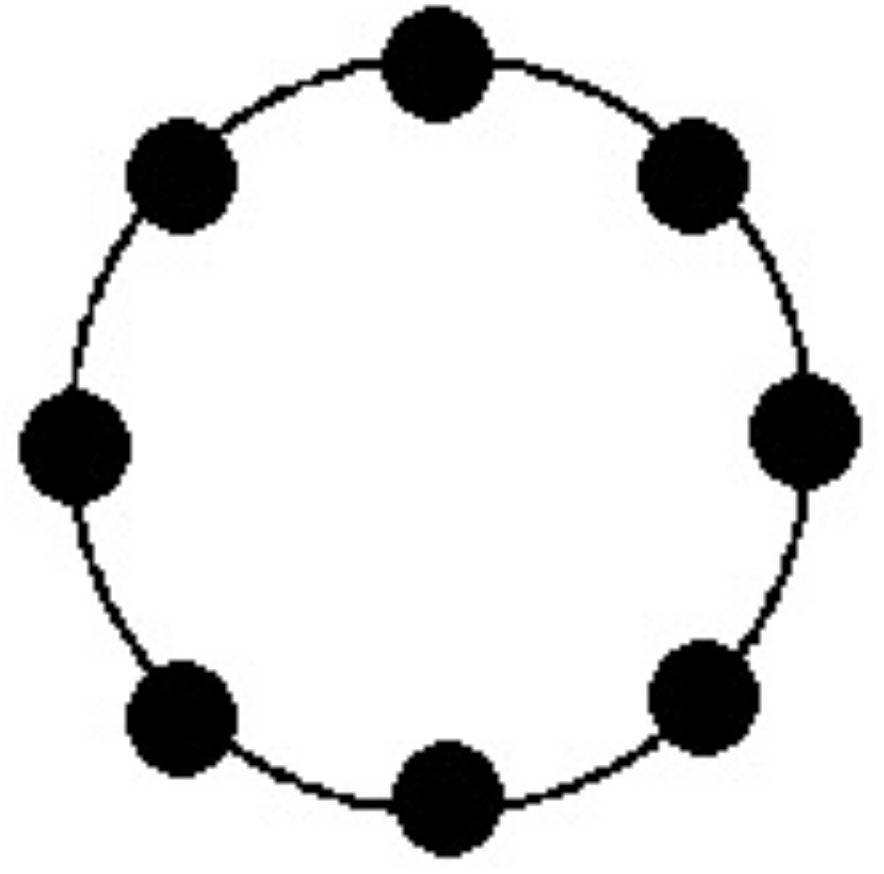
\includegraphics[scale=0.11]{../figures/ring.png}
\end{center}
Il \textbf{ring} è un array lineare chiuso su stesso (dove si sono collegati i nodi estremi, cioè quelli con grado 1). Il grado diventa quindi 2 per tutti i nodi. 
Il diametro subisce la prima caratteristica fondamentale del ring: per raggiungere un dato nodo si hanno a disposizione due direzioni anziché una, per cui il diametro complessivo è $\frac{N}{2}$.

Anche la tolleranza ai guasti migliora, in quanto un nodo guasto non pregiudica necesssariamente l'integrità del sistema (ne servono 2 per isolare una parte della rete).

\subsubsection{Connessione completa}
\begin{center}
	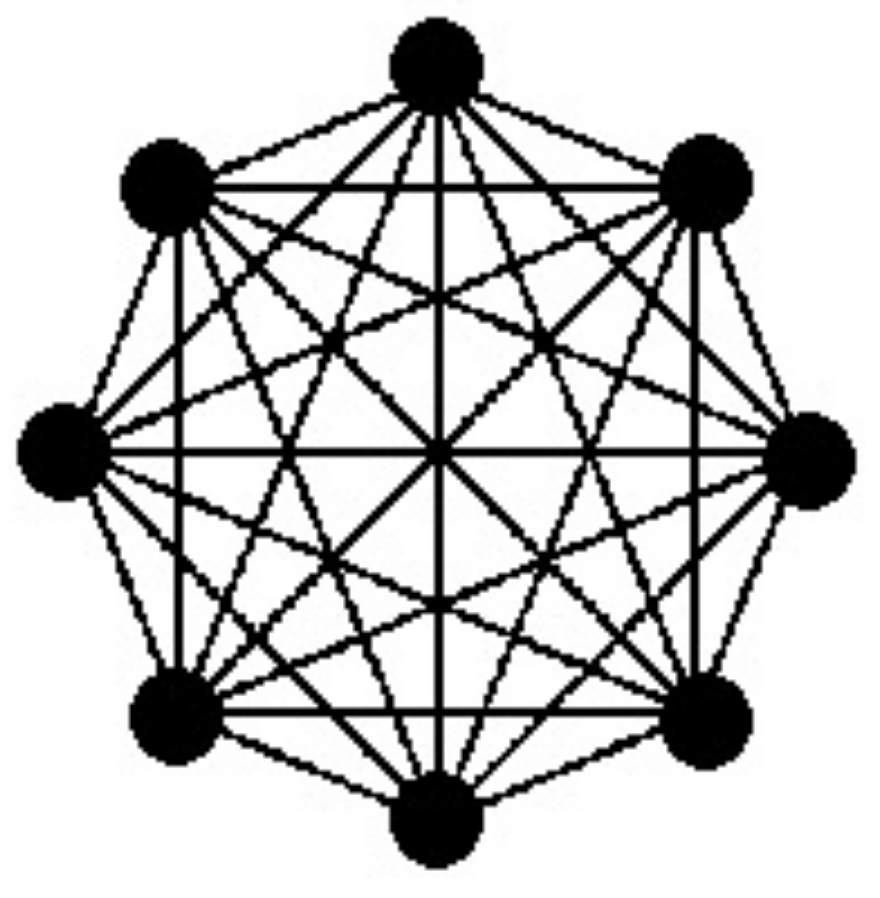
\includegraphics[scale=0.12]{../figures/full_conn.png}
\end{center}
La \textbf{connessione completa} (o \textit{tutti-a-tutti}) è la rete di interconnessione più, appunto, \textit{connessa}, che vediamo.
In questo caso ogni nodo comunica direttamente con ogni altro nodo: il grado è per tutti i nodi $N - 1$ e il diametro è 1 (si arriva direttamente al nodo desiderato).
Svantaggioso è chiaramente il numero totale di link, che cresce come $N \frac{N - 1}{2}$: l'approccio chiaramente non è scalabile!

Dobbiamo quindi trovare modelli per reti di interconnessione che presentino parte dei vantaggi della connessione completa (alta tolleranza ai guasti, bassissimo diametro), riducendo però il numero di link e quindi aumentando la scalabilità.

\subsubsection{Albero binario}
\begin{center}
	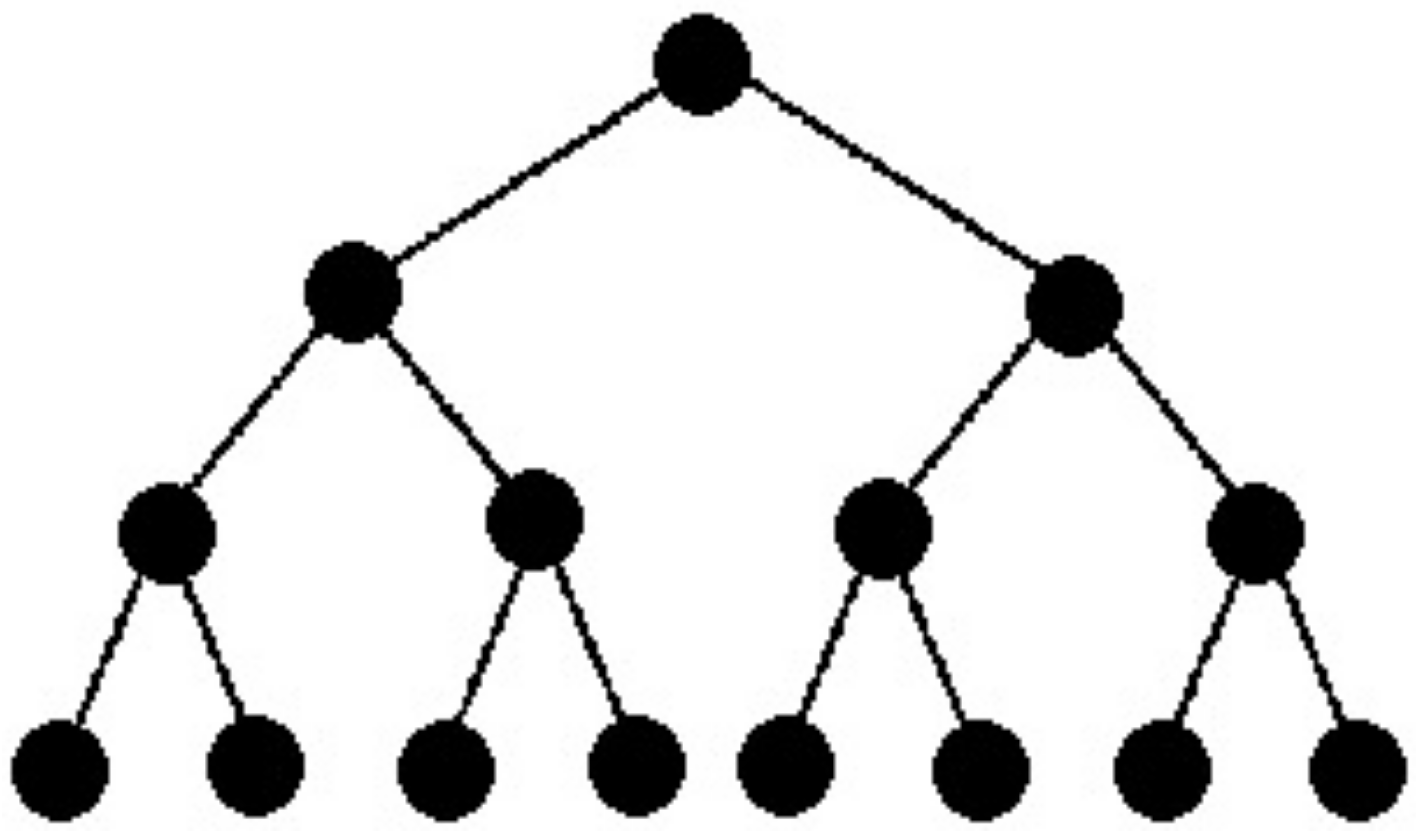
\includegraphics[scale=0.11]{../figures/btree.png}
\end{center}
Si può pensare di ordinare i nodi secondo un \textbf{albero binario}.
In questo caso vorremo definire l'\textit{altezza} dell'albero come $h = \log_2(N)$ per $N$ nodi e i gradi come:
\begin{itemize}
	\item 2 per la radice;
	\item 1 per le foglie;
	\item 3 per tutti gli altri nodi.
\end{itemize}
Il diametro sarà (senza dimostrazione) $2 \times (h - 1)$ e il numero totale di link $N - 1$ ($O(N)$ anziché $O(N^2)$, già migliore).

Questo tipo di rete permette una facile comunicazione fra nodi sugli stessi sottoalberi, mentre per comunicazioni fra sottoalberi distinti porta alla \textit{congestione dei rami alti}: questo la rende poco scalabile.
In particolare, più ci avviciniamo alla radice minori saranno i link (e quindi maggiore il carico sul singolo link). Inoltre, i nodi dovranno fare da router, e quindi più ci avviciniamo alla radice più i nodi hanno responsabilità di router sempre maggiori.
Questo culmina sulla radice stessa, che chiaramente è sottoposta ad un carico non indifferente e rappresenta il punto più debole dell'architettura ad albero binario.

Per quanto riguarda la tolleranza ai guasti, vale lo stesso discorso: più in alto (verso la radice) avviene il guasto, maggiori sono le conseguenze per il sistema. Come caso limite, se si guasta la radice si incorre in un partizionamento in due dell'intero sistema.

Soluzioni alternative si possono avere sfruttando alberi, anziche binari, \textit{$n$-ari}, cioè con $n$ figli per nodo.

\subsubsection{Stella}
\begin{center}
	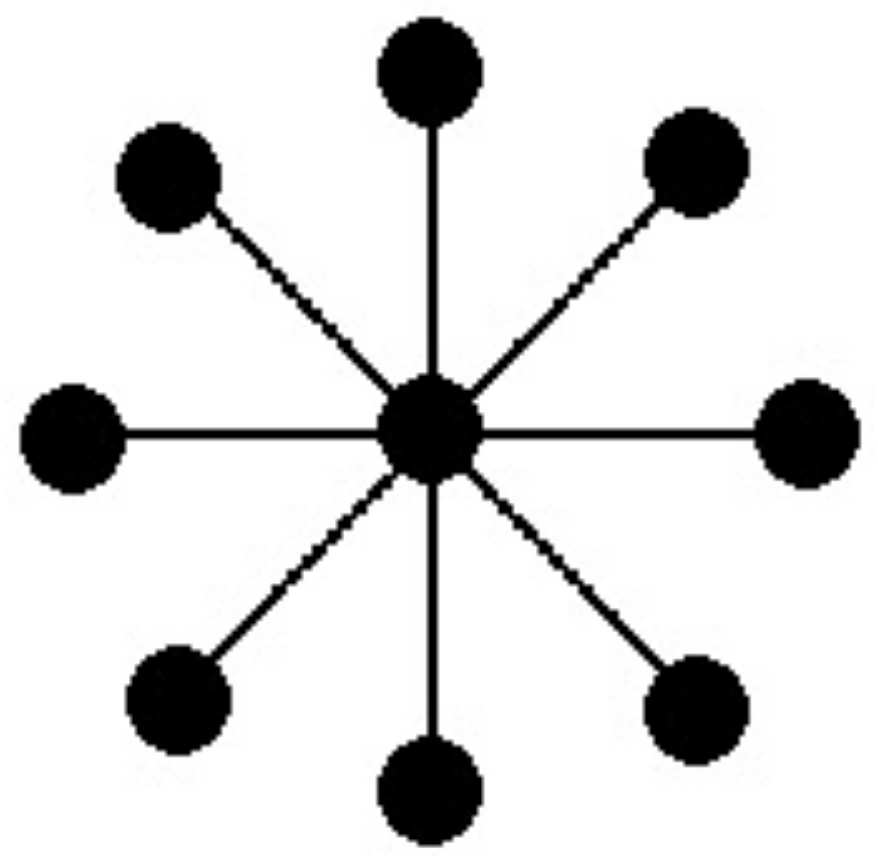
\includegraphics[scale=0.11]{../figures/star.png}
\end{center}
Le reti di interconnessione a \textbf{stella} prevedono un singolo nodo centrale che connette $n-1$ nodi periferici.
Il grado di tale nodo centrale sarà quindi $n - 1$, mentre i nodi periferici avranno 1.
Il diametro sarà 2 (dobbiamo passare sempre dal nodo centrale, a meno che non si voglia parlare col nodo centrale stesso).
Il numero di link è ridotto ($N - 1$), e quindi da questo punto di vista il sistema è vantaggioso.

Il difetto più grande è chiaramente la presenza di un singolo nodo centralizzato soggetto a guasti o sovraccarichi.
Questo è il classico problema del \textit{single point of failure} delle architetture client-server: possiamo infatti intendere il nodo centrale come un \textit{server} e i nodi periferici come \textit{client} di tale server.

Abbiamo quindi che per quanto si possa rendere potente il nodo server, questo dovrà portare tutto il carico della rete (bassa scalabilità), e un guasto del server rappresenterà una mancanza di servizio per tutti i nodi client (bassa robustezza).

\subsubsection{Mesh bidimensionale}
\begin{center}
	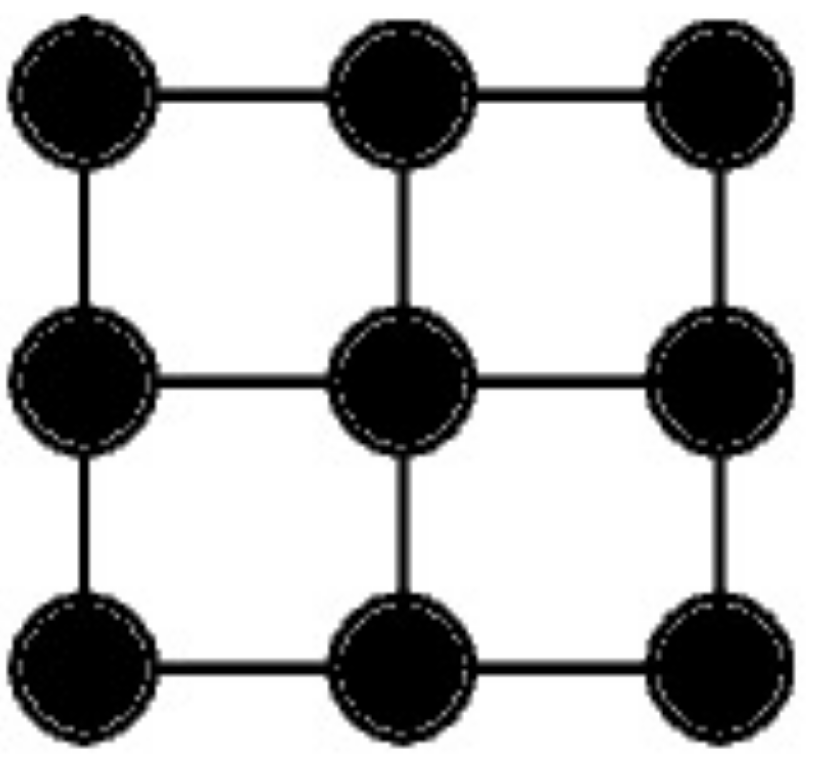
\includegraphics[scale=0.09]{../figures/mesh.png}
\end{center}
La struttura a \textbf{mesh bidimensionale} prevede di disporre i nodi su una griglia bidimensionale.
In questo caso il lato della griglia sarà $r = \sqrt{N}$ e il grado dei nodi sarà:
\begin{itemize}
	\item 2 per i nodi ai vertici,
	\item 3 per in nodi \textit{"centrali"} ai lati (diciamo nodi agli \textit{spigoli});
	\item 4 per tutti gli altri nodi.
\end{itemize}
Il diametro sarà $2 \times (r - 1)$, e il numero totale di link ($2 \times (n - 2) \times r$).

La resistenza ai guasti di queste configurazioni è buona, ma può essere milgiorata. Vediamo come.

\subsubsection{Toro bidimensionale}
\begin{center}
	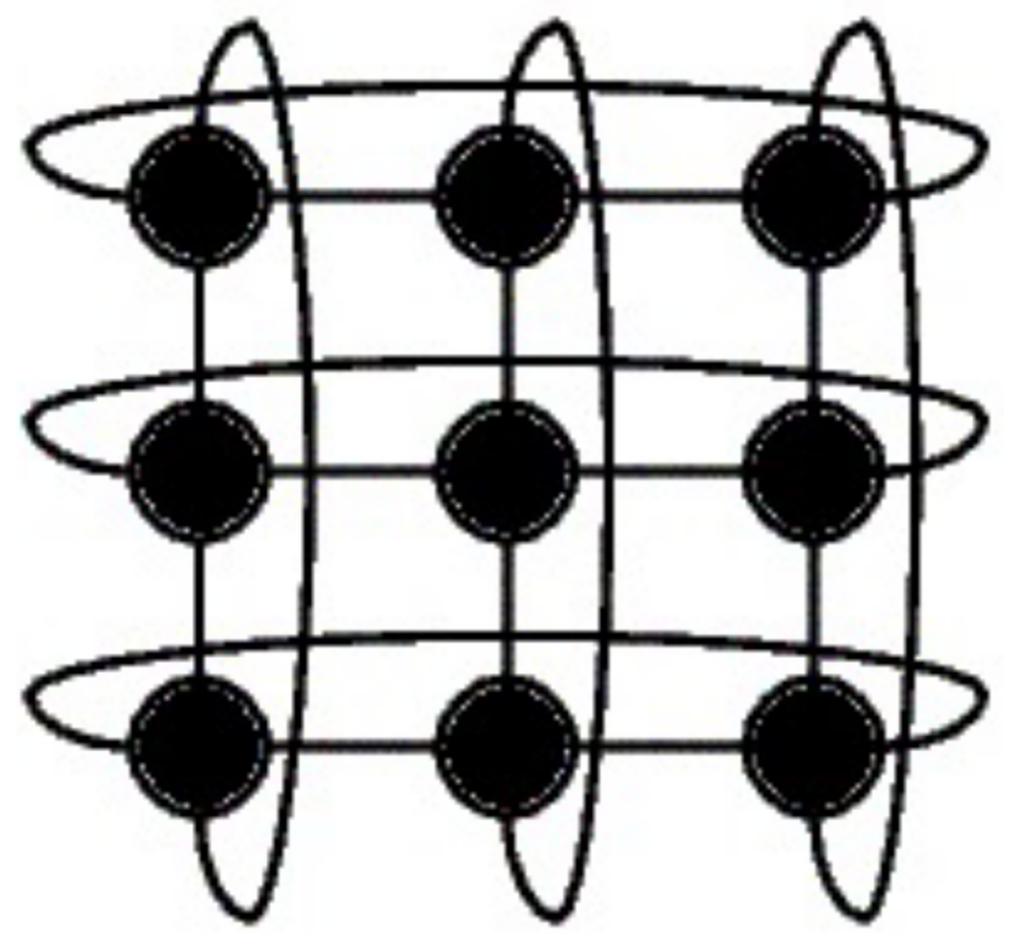
\includegraphics[scale=0.1]{../figures/torus.png}
\end{center}
Collegando i nodi ai lati opposti di una struttura a mesh bidimensionale si ottiene una struttura a \textbf{toro bidimensionale}.
In questo caso il grado è 4 per tutti i nodi, ma il diametro migliora: va sostanzialemente come $r$ (dove $r$ è il lato calcolato come $r = \sqrt{N}$, uguale alla rete bidimensionale).
Il numero totale di link è invece stabile a $2N$.

Questa topologia risulta ben scalabile e notevolmente resistente ai guasti: sostanzialmente rappresenta per la mesh bidimensionale quello che il ring rappresenta per l'array lineare.

\par\medskip

Architetture come le ultime viste (mesh, tori, ecc...) possono essere estese a più dimensioni, portando a \textit{ipercubi}, \textit{ipertori}, ecc... 

\subsection{Metriche di prestazione}
Finiamo questa sezione del programma parlando di alcune \textbf{metriche} per le \textbf{prestazioni} di architetture descritte secondo la tassonomia di Flynn.

\begin{itemize}
	\item Chiamiamo \textbf{speed-up} ($S$) il rapporto fra il tempo di esecuzione sequenziale sul tempo di esecuzione parallelo (SIMD o MIMD, cioè):
		$$
			S = \frac{T_1}{T_N}
		$$

		Questa metrica rappresenta quindi il \textit{guadagno} in velocità che si ha passando ad un sistema multiprocessore. Idealmente vorremmo $S = N$, cioè \textit{lineare} col numero di unità di elaborazione, ma come vedremo a causa dell'overhead introdotto da più processori dobbiamo accontentarci di $S < N$, con $S \approx N$.

		l valore dello speed-up dipende dalle applicazioni, ma anche dall’architettura: nelle SIMD spesso $S \approx N$, mentre nelle MIMD è difficile far crescere $S$ (non è facile far lavorare pienamente tutte le CPU, o trasferire efficientemente fra di esse).

	\item L'\textbf{efficienza} ($E$) è invece definita come lo speed-up sul numero di unità di elaborazione, cioè:
		$$
			E = \frac{S}{N}
		$$
		Come prima, vorremmo $E = 1$, ma dobbiamo accontentarci di $E < 1$, con $E \approx 1$.
\end{itemize}

Per giustificare come mai non si può mai avere $S = N$ (o equivalentemente, $E = 1$), ci viene incontro la \textit{legge di Amdhal}.
Questa dice che un parallelismo \textit{"perfetto"} (nelle varie attività compiute da un calcolatore) non è mai raggiungibile in quanto saranno \textit{sempre} presenti sequenza di programmi \textit{intrinsecamente seriali}.
Semplificando, si può dire che ci saranno sempre degli intervalli di tempo sequenziale ($T_\text{seq}$), impiegati ad eseguire istruzioni non parallelizzabili come operazioni di I/O, costrutti condizionali, algoritmi intrinsecamente sequenziali, ecc....

Più nello specifico, la legge di Amdahl ridefinisce lo speed-up come:
$$
S = \frac{T_1}{T_{\text{seq}} + \frac{T_1 - T_\text{seq}}{N} }
$$
cioè il guadagno di speed-up è dato solo dalle parti parallelizzabili del programma ($T_1 - T_\text{seq}$), mentre le parti seriali ($T_\text{seq}$) non hanno grandi guadagni.

Il problema è che, prendendo il limite per $N \rightarrow \infty$, si ha:
$$
\lim_{N \rightarrow \infty} S = \lim_{N \rightarrow \infty} \frac{T_1}{T_{\text{seq}} + \frac{T_1 - T_\text{seq}}{N} } = \frac{T_1}{T_\text{seq}}
$$
cioè a dominare lo speed-up sono le parti sequenziali (le parti non sequenziali vengono abbattute velocemente, quelle sequenziali mai e rimangono come overhead complessivo dell'intero sistema).

\subsubsection{Multitasking}

In conclusione, vogliamo dire che il \textit{multitasking} è quasi sempre vantaggioso (anche intuitivamente), ed è di notevole importanza anche nelle macchine per mantere alto lo sfruttamento delle CPU (ciò che avevamo chiamato \textit{efficienza CPU}).

Il vincolo che vogliamo rispettare sarà, quindi, di base:
$$
P >> N
$$
cioè avere più processi che unità di elaborazione. 

\subsection{Sincronizzazione processi}
Iniziamo quindi a vedere la \textbf{sincronizzazione} fra processi, in particolare con riferimento ai \textit{tipi} di interazione che ci possono essere fra processi, e i problemi di \textbf{mutua esclusione} e \textbf{sincronizzazione}.

\subsubsection{Tipi di interazione}
Ricordiamo che i processi possono interagire fra di loro secondo 2 modalità:
\begin{itemize}
	\item \textbf{Cooperazione}: quindi per sincronizzazione diretta o esplicita, cioè definita dai programmi;
	\item \textbf{Competizione}: quindi per sincronizzazione indiretta o implicita, non definita dal codice dei programmi ma causata da tentativi di accesso \textit{simultaneo} a risorse limitati. 
\end{itemize}

Nominiamo poi l'\textbf{interferenza}, rappresentata da errori dipendenti dal tempo.

Per l'interazione fra processi faremo riferimento a 2 modelli principali:
\begin{itemize}
	\item A \textbf{memoria comune}: in questo caso prevediamo $n$ processi con risorse private (cioè spazi di indirizzamento privati per ognuno), ma che possono accedere a risorse \textit{condivise} in un terzo spazio di indirizzamento comune per tutti. 

		Se vogliamo ricondurci alla tassonomia di Flynn, questo è un esempio di macchina multiprocessore (o monoprocessore in \textit{timesharing}...) di tipo MIMD (se vogliamo SM-MIMD): più unità di elaborazione sugli stessi dati (tralasciando il fatto che ogni unità ha poi i suoi dati privati);

	\item A \textbf{scambio di messaggi}: in questo caso prevediamo $n$ processi in esecuzione su unità di elaborazione distinte (ancora, multiprocessore o monoprocessore in \textit{timesharing}) con le loro risorse (memorie) locali, che possono comunicare fra di loro attraverso un meccanismo di \textit{scambio di messaggi}.

Notiamo di nuovo che non è necessario che le unità siano necessariamente distinte, e ricordiamo che non sono i processi a comunicare in sé per sé, ma le unità di elaborazione a supportare un meccanismo che permette tale comunicazione.

		Questo è sempre un esempio di architettura MIMD (se vogliamo DM-MIMD), simile ad esempio a quella che ci permettono i sistemi multicalcolatore connessi in rete (più macchine distinte, con le loro risorse, che comunicano fra di loro).
\end{itemize}



\end{document}
